\chapter{Proposed approach} % Main chapter title

\label{chapter::approach} % Change X to a consecutive number; for referencing this chapter elsewhere, use \ref{ChapterX}

\lhead{Chapter 3. \emph{Proposed approach}} 

This section presents an overview of our online ensemble
tracking approach, and then describe the details of each stage of our
processing pipeline. Given tracking inputs, the algorithm estimates the
trajectory of an object as it moves around a scene. The tracker outputs labels
of the tracked object in every frame of the video \ref{fig::global_diagram}.
These labels provide position and scale information for evaluation and analysis.

\begin{figure}[h!]
\centering
\includegraphics[page=2, width=0.8\linewidth, trim= 0cm 5.1cm 6cm 5.3cm,
                 clip=true]{Figures/global_diagram}
\caption[Tracking diagram]{\small Tracking diagram. The proposed system takes
        initial bounding box, image sequences and the list of trackers as inputs.
        After tracking ensemble, the system drops out tracking results for each
        frame.}
\label{fig::global_diagram}
\end{figure}


\section{Overview}

We illustrate the main components of our method in
Figure \ref{fig::diagram}.
%Generic single-object tracking could be defined as the localization of an
%object through a video sequence. It is generic because the system is able to
%track any kind of object (faces, cars, etc.), and is single because the system
%will track just one object and not many at the same time. This section details
%all the components for our ensemble approach.
%The proposed approach in this paper is illustrated in figure \ref{fig::diagram}.
At each frame, our method proceeds as follows.
First, we independently run all trackers
$T = \{ t_1, t_2, ..., t_n \}$
in a pool of size $n$, which produce a set of predicted target
states
$X = \{ x_1, x_2, ..., x_n \}$ (Fig.~\ref{fig::diagram}a).
These predictions are the raw input of our ensemble algorithm,
and may be in the form of bounding boxes. A bounding box is here defines as the
set of pixels covered by a rectangular area.
Our ensemble methodology then looks for spatial coherence among the predicted
target states, and verifies the appearance of the predicted image regions
with respect to an object model
%associated to each predicted state
(Fig.~\ref{fig::diagram}b). The idea is that for a given frame,
we would like to discover the subset of trackers that are correctly
estimating the target state and to ignore all erroneous predictions.
The result is a selection of inlier tracking predictions
that contain the object with high confidence
(Fig.~\ref{fig::diagram}c).
A final ensemble prediciton of the target state is then derived from
these inlier estimations (Fig.~\ref{fig::diagram}d).
Finally, we use the prediction of the ensemble to update a model of the
target appearance, and periodically reinitialize outlier trackers
(Fig.~\ref{fig::diagram}e).
This entire process is then repeated for each new frame in the video sequence.

\begin{figure*}[t!]
\centering
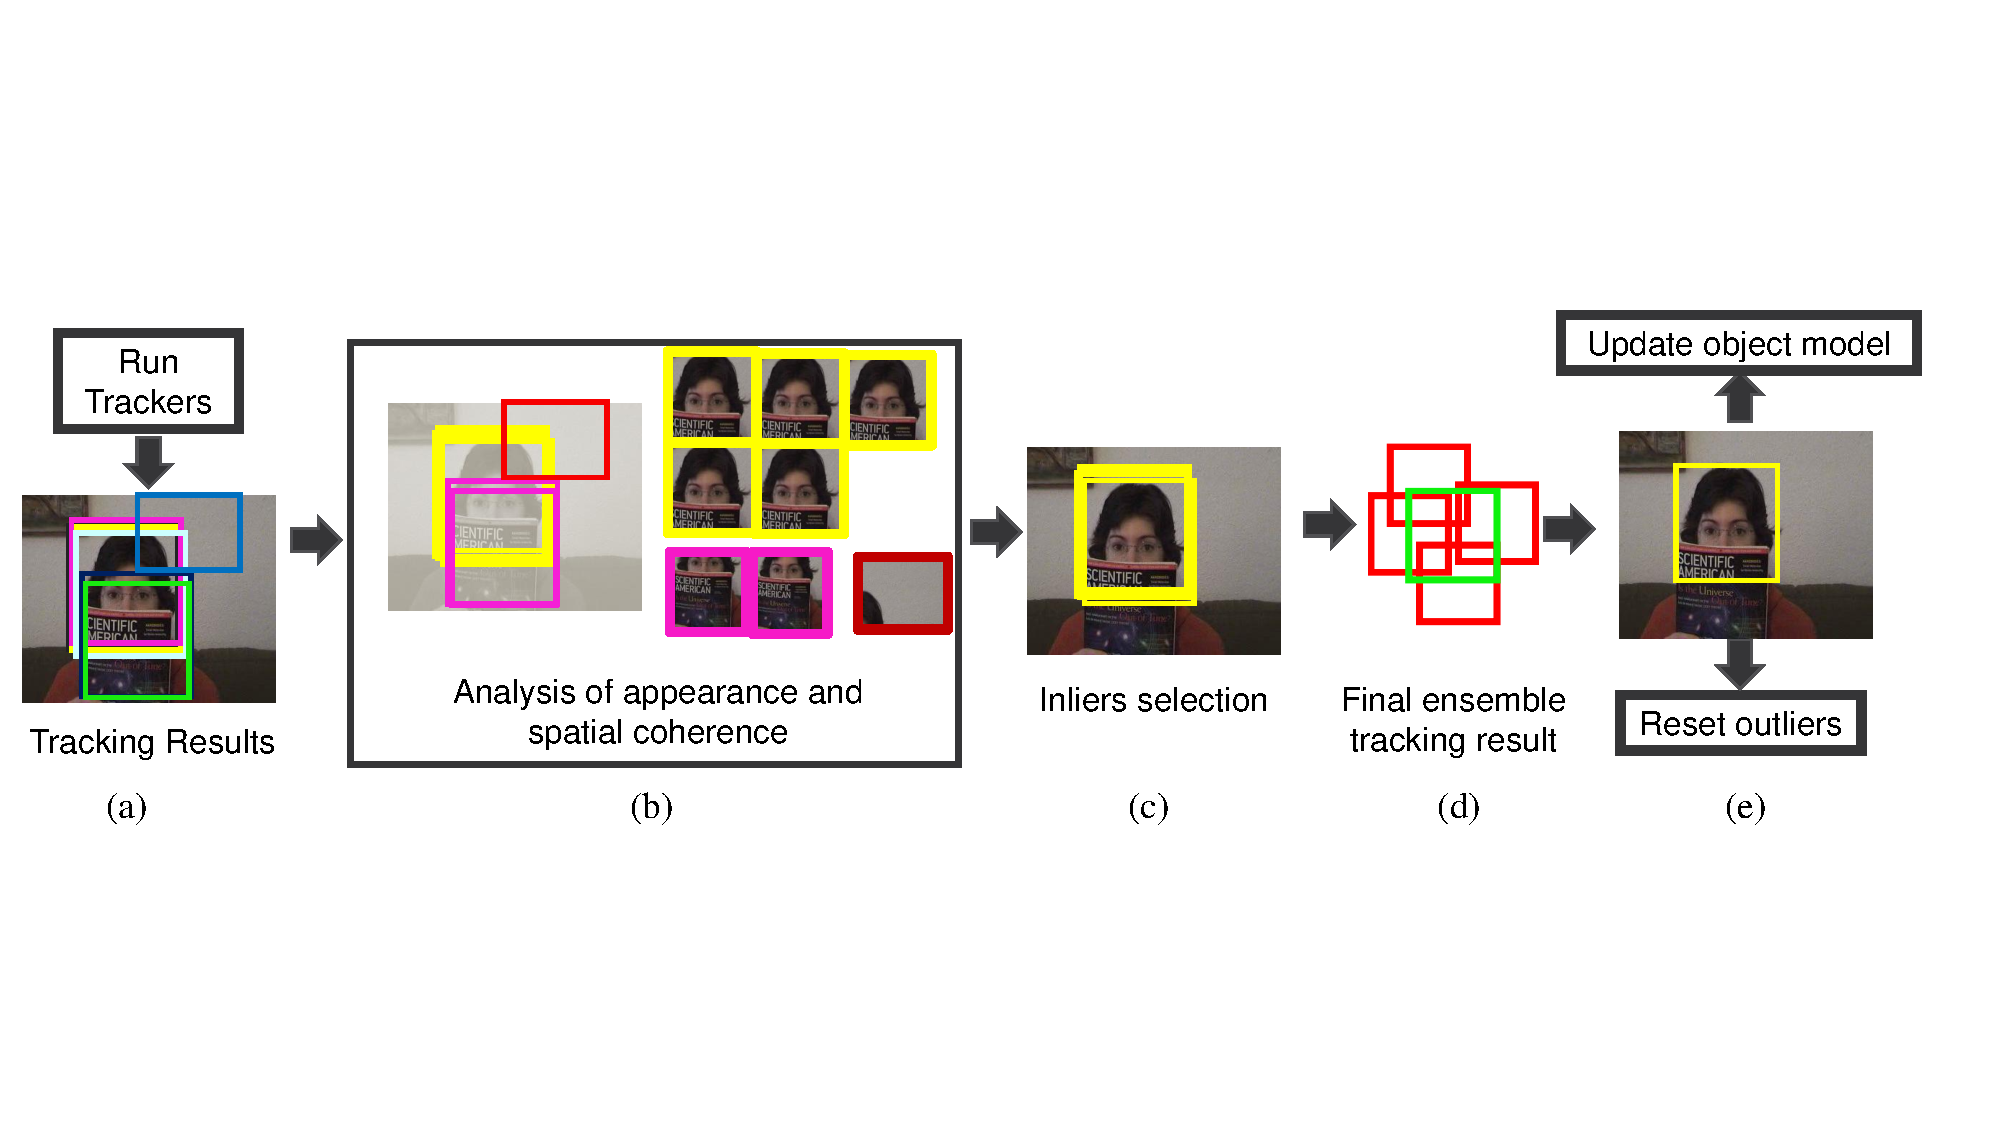
\includegraphics[width=1\linewidth, trim= 0cm 5.1cm 1.3cm 5.3cm, clip=true]{Figures/diagram}
\caption [Proposed methodology.]
    {\small Basic diagram of our approach. On each frame, we analyze coherence
        between tracking results. We apply spatial and appearance models with
        the goal of finding inliers. Then, we select best tracker that follows
        the target. Finally, we reset outliers and  update object model on
        necessary cases.
}
\label{fig::diagram}
\end{figure*}


In spite of the simplicity of our ensemble procedure, our experiments
evidence that the ensemble is able to produce more accurate tracking results
than any of the trackers in the pool. Furthermore, the ensemble can
achieve state-of-the-art performance on benchmarking videos.

In the following, we provide the details of each processing stage and their
role in the overall ensemble procedure.

%Such appearance and spatial anylisis produces a set of inlier estimates
%analyzes these predicted states
%Then, our method clusters the predicted states $X$ into a set of
%This input corresponds to the initial rectangular box for an object in a
%sequence.
%All trackers are initalized and an object model is created.
%Then, on each frame, our method runs and groups all trackers results by
%position into a set of
%Also, we obtain a similarity measure which compares an actually tracking result
%patch to the current object model. The output should be the probabilities of
%similarity between the object model and each tracker result in that frame
%$S = \left \{ s_1, s_2, ..., s_n \right \}$.
%The system selects cluster that best follows the object $c^*$.
%This selection is
%performed using two criterias: Cluster with highest number of members, or
%cluster with highest similarity measure. Remaining groups are considered
%outliers and members are reinitialized each 15 frames.

\section{Analysis of appearance and spatial coherence}
After running all trackers in the pool, our method uses their state estimates
$X$ as input of the appearance and spatial coherence stage
(Fig.~\ref{fig::diagram}b). The goal is to determine the set of
trackers that correctly estimate the true target state. We denote these trackers
as inliners in Fig.~\ref{fig::diagram}c.

In order to achieve this, we note a simple but key observation: in most cases,
there is only a small subset of trackers that fail to correctly track the
object in any given frame.
In such scenario, the majority of the trackers focus correctly in the object,
and we could use clustering techniques to automatically determine this set
of inlier trackers.
A more difficult scenario is when most of the trackers fail, but only a few
focus in the correct image region. But even in this case, tracker failures
tend to be distributed in varied image locations, while the few correct
trackers focus on a spatially coherent region. Once again, spatial clustering
of the locations $X$ can help discover the underlying true object location.
In an extreme scenario, when only one tracker correctly follows the object,
we can no longer rely on spatial clustering alone.
A complementary cue can be introduced to overcome this issue: a target
appearance model. We therefore explore the use of these two cues
to select a subset of inlier trackers that follow the object region with
high confidence.

%But even if a majority of the trackers fail in a given frame,
%In this stage, our approach takes as inputs all trackers bounding boxes results.
%Using spatial information, we are able to create groups of trackers whose
%members have affinity in position and scale. Also, from each bounding box $x_i$,
%we extract patches and compute similarity score $s_i$ with an object model.

\subsection{Spatial clustering.}

Cluster analysis is the formal study of algorithms and methods for grouping, or
classifying objects. These objects are described as a set of measurements or by
relationships between the object and other objects. A \textit{cluster} is
comprised of a number of similar objects collected or group together. Other
authors define a cluster as a set of entities which are alike, and entities from
different clusters are not alike, or "A cluster is an aggregation of points in
the test space such that the \textit{distance} between any two points in the
cluster is less than the distance between any point in the cluster and any point
not in it" \cite{Jain88}.

\begin{figure}[b!]
\centering
\includegraphics[page=4, width=0.9\linewidth, trim= 0.4cm 5.5cm 6.5cm 5cm,
                 clip=true]{Figures/global_diagram}
\caption[Spatial clustering stage]{\small Spatial clustering stage. Using
        trackers estimate, we cluster similar bounding boxes using equation
        \ref{eq::diff}. On right image, each color represents a cluster.}
\label{fig::clustering}
\end{figure}

Cluster analysis is the process of classifying objects into subsets that have
meaning in the context of a particular problem. The objects are thereby
organized into an efficient representation that characterizes the data.
Clustering methods require that an index of proximity, or alikeness, or
affinity, or association be established between pairs or patterns. A
\textit{proximity matrix} $|d(i, j)|$ accumulates the pairwise indices of
proximity in a matrix in which each row and column represents a pattern.
Diagonal entries of a proximity matrix are ignored since all paterns are
assumed to have the same degree of proximity with themselves. Also it is
assumed that all proximity matrices are symmetric, so all pairs of objects have
the same proximity index, independent of the order in which they are written.A
proximity index is either a \textit{similarity} or a \textit{dissimilarity}.
The more the \textit{i}th and \textit{j}th objects are similar one another, the
larger a similarity index and the dissimilarity index are.

At this stage, we perform spatial clustering of all tracker predictions $X$.
Bounding boxes with large overlap, similar location and scale should be grouped
into the same cluster.
Since we do not know the number of natural groups beforehand, we use
an agglomerative clustering technique to achieve this. In practice,
we apply complete-link hierarchical agglomerative clustering (CL)
\cite{Jain88}.
We define a dissimilarity measure between pairs of bounding boxes equal to:

\begin{equation}
d(x_i,x_j) = 1 - \frac{|x_i \bigcap x_j|}{|x_i \bigcup  x_j|}
\label{eq::diff}
\end{equation}

Using all dissimilarity values, we construct a symmetric $n \times n$ proximity
matrix $D$. In CL, a pair of bounding boxes $(x_i, x_j)$ will be grouped in
the same cluster if their dissimilarity is below some threshold $v$.
For all our experiments we set this value to $0.8$.
The result of CL is a grouping of the input bounding boxes $X$ into 
$m$ clusters $C = \left \{ c_1, c_2, ..., c_m \right \}$,
which are illustrated with colors in Fig.~\ref{fig::diagram}b. These clusters
satisfy the following:
\begin{itemize}
\item $c_i \cap c_j = \emptyset$ for $i$ and $j$ from 1 to $m$, $i \neq j$
\item $c_1 \cup c_2 \cup ... \cup c_m = T$
\end{itemize}

\subsection{Object modeling.}
Visual object tracking has been formulated as a tracking-by-detection problem
recently. Object modeling is dynamically performed to support object detection
over all frames. Mostly all the approaches can be classified into two categories:
\textit{Generative appearance models}, that mainly focus on how fit the data into
their correspondent object class; and \textit{discriminative appearance models},
which assume object tracking as a binary classification issue. Main goal is to
maximize the separability between object and non-object regions discriminately.

\begin{figure}[t!]
\centering
\includegraphics[page=3, width=1\linewidth, trim= 0.4cm 9.9cm 7.5cm 1.8cm,
                 clip=true]{Figures/global_diagram}
\caption[Patches and features extraction process]
{\small Patches and features extraction process. For a given patch, Histograms
of Oriented Gradients are extracted. The final result, corresponds to a hog
descriptor.
}
\label{fig::features_extraction}
\end{figure}

Generally, Discriminative methods train a classifier using data acquired from
previous frames, and subsequently use the trained classifier to evaluate
possible object regions at the current frame. After localization, a set of
\textit{positive} and \textit{negative} samples are heuristically selected to
update the classifier. Some approaches apply online boosting
\cite{Babenko2010,Grabner2008,Grabner2006}, that make a discriminative
evaluation of features taken from a candidate feature pool, and then select the
top ranked features to conduct the tracking process. Other methods apply
Support Vector Nachines (SVM) method, which learns a margin-based discriminative
appearance model, in order to maximize inter-class separability. These
classifiers are trained using visual representations of the object.

At this stage, we would like to verify the appearance of all tracker
predictions $X$ in comparison to an object appearance model.
In order to do so, we train an appearance classifier that aims at separating
positive target bounding boxes from background bounding boxes.
We extract positive samples from the target location given at the first frame
and also from uniformly sampling background bounding boxes around the target
bounding box.
In practice, we adopt a feature representation based on HOG and a SVM
classifier with probability outputs.
Using the classifier, we compute appearance scores  
%During tracking loop,
%from each tracker bounding box, we extract it correspondent image patch
%and evaluate in object model.
%On each frame, we obtain probability scores
$S = \left \{ s_1, s_2, ..., s_n \right \}$ for each tracking result $x_i$ in
$X$ (Figure \ref{fig::svm_app}). We considered this model, because other methods found in 
\cite{zhang2014meem,Bai2013}, obtained better results. Also, HOG features are
more robust to deformable objects than other image features used in
tracking-by-detection methods \eg Haar.
%We considered a probability score as a similarity measure which compares a tracker
%patch with the object model in the current frame. 

\begin{figure}[b!]
\centering
\includegraphics[page=5, width=1\linewidth, trim= 0.4cm 5.5cm 0cm 5cm,
                 clip=true]{Figures/global_diagram}
\caption[Appearance estimation for trackers estimates.]
        {\small Appearance estimation for trackers estimates. On each frame,
        We compute appearance score for each tracker result using a previously
        trained classifier. We adopted HOG as image features.}
\label{fig::svm_app}
\end{figure}


\iffalse
In our approach, we are asumming that target object is detected at the
beginning of tracking process. This image region is considered to be a positive
image sample for the classification model. We also extract negative samples
creating random regions of the same size as the positive sample. Finally, we
create an object model taking these labeled samples and training a classifier.
We adopted HOG as image features representation and SVM for classification
model. 
\fi

\section{Selection of inliers}
\label{sec:inliers}
The clustering stage and appearance scoring provide cues about which trackers
can be considered as correctly tracking the target.
We evalute two simple criteria that optimally select a group of trackers as
inliers (Fig.~\ref{fig::diagram}c).
In our experiments, we consider cluster size and appearance scores as
potential cues to select inliers.

%After performing clustering stage and obtaining classification scores for each
%tracker, we can select the cluster that best follows the object. We present two
%selection criterias for inliers.

\textbf{Cluster size:}
This critera follows the idea that the largest spatially coherent cluster
is associated to the true target location. Therefore, we flag all trackers
in the largest cluster as inliners, and all other trackers as outliers.

\begin{equation}
 c^{*} = \argmax_{c_i\in C} |c_i|
\end{equation}

%Once groups are
%formed, we search the cluster $c^{*}$ in the list of clusters $C$ of size $m$,
%with highest members number. 
%\begin{equation}
%c^{*} = \arg\max_{c_i\in C} ~\sum_{t \in c_i}t_i 
%\end{equation}

\textbf{Appearance scores:}
In this criteria, we trust our object appereance model to validate if a cluster
contains bounding boxes that focus on the true target location.
To do so, we max-pool the appereance scores $s$ of the bounding boxes $x$ within
each cluster:
%In this case we are
%considering classification scores for each cluster. Each cluster gives a score
%per cluster. Then, we select the winner cluster whose score is the highest one. 
\begin{equation}
 c^{*} = \argmax_{c_i\in C} \max_{x_j \in c_i} s_{j}
\end{equation}

%where $m_i \in M = \left \{ m_1, m_2, ..., m_m \right \}$ corresponds to maximum
%score value of $c_i$ cluster \J{Pooling}:
%\begin{equation}
%M =  \left \{ \max_{s\in S} s_i \in c_i \right \}
%\end{equation}
\iffalse
One common issue that most of tracking-by-detection methods deal with,
corresponds to when is important to update object model.
Considering model too adaptive, increases risk of contaminating object model
with spurious samples. In other cases, not including important object
information into the model, tracking fails due to natural appearance changes
\eg face rotations. In our approach, we consider to update object model, if
$c^*$ score is higher than a threshold value $w$. For experiments we set $w$
the value of 0.3.
%\eg face rotations. In our approach, we consider to that if $c^*$ score is higher
%that a threshold value $w$, object model is updated. In experiments we set $w$
%the value of 0.3.
\fi

\begin{figure*}[t!]
\centering
    \figuresp{trackers/027.jpeg}
    \figuresp{trackers/028.jpeg}
    \figuresp{trackers/029.jpeg}
    \figuresp{trackers/030.jpeg}
    \figuresp{trackers/031.jpeg} 

    \vspace{0.15cm}

    \figuresp{clusters/027.jpeg}
    \figuresp{clusters/028.jpeg}
    \figuresp{clusters/029.jpeg}
    \figuresp{clusters/030.jpeg}
    \figuresp{clusters/031.jpeg}  

    \vspace{0.15cm}

    \figuresp{final_result/027.jpeg}
    \figuresp{final_result/028.jpeg}
    \figuresp{final_result/029.jpeg}
    \figuresp{final_result/030.jpeg}
    \figuresp{final_result/031.jpeg}


\caption{\small System behavior in five frames. Given image input, trackers will
give results on where the object might be (first row). Then, all results are
clustered using hierarchical agglomerative clustering (second row). We focus on
selecting the group with highest number of members, or cluster with best
appearance score (third row). Finally, we reinitialize outliers.}   
\end{figure*}


\section{Final ensemble tracking result}
In order to provide an estimation of the state of the target using our
ensemble, we fuse the outputs of all inlier trackers from the previous stage.
There are multiple choices on how to impĺement this fusion. For example,
it can be a linear combination of the inlier bounding boxes. In practice,
we use a simpler approach that selects the medoid bounding box as the final
ensemble output. That is, we output a
bounding box $x^{*}$
whose sum of distances with the rest of inlier bounding boxes
is minimum:
\begin{equation}
x^{*} = \argmin_{x_{i} \in c^*}  ~\sum_{x_{j} \in c^{*}}d(x_{i}, x_{j}) 
\end{equation}

\section{Model update and outlier reset}
Once our ensemble estimates the target state, we can proceed to update the
object model and steer failed trackers in the pool.

\begin{figure}[b!]
\centering
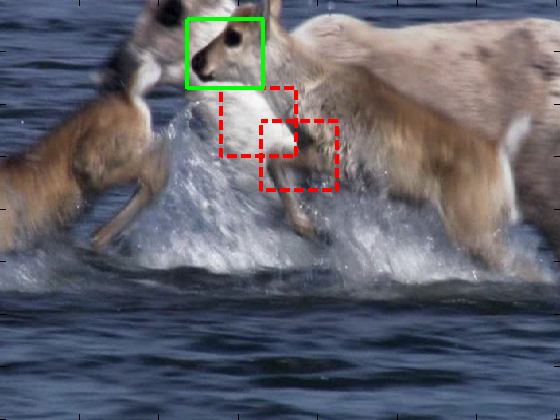
\includegraphics[width=0.5\textwidth]{Figures/clustering/deer_outliers.png}
\caption[Outliers reinitialization]{Outliers reinitialization. In this Figure,
dashed red bounding boxes are tagged as outliers. These trackers states are
reset to the latest target state prediction from the ensemble (green bounding
box.)}
\label{fig::outliers}
\end{figure}

The first goal of this final stage is to keep our target appearance model
updated. In order to avoid model drifting, we only update the appearance
model periodically when our tracking ensemble has high confidence in the
selection of inliers. Such confidence can be measured using the appearance
scores $S$ or the percentage of trackers in the inliner cluster.
When confidence is high, a image patch is extracted at the predicted
location and provided as a new positive sample to retrain or update
our object appearance model.

The second goal is to steer failed trackers in the pool back to the target.
When a tracker is consistently tagged as an outlier, our algorithm automatically
resets its state to the latest target state prediction from the ensemble
(Figure~\ref{fig::outliers}).
This reinitialization procedure is only performed periodically every 15 frames
so that we can also take advantage of the capability of some trackers
to recover from short-term tracking failures.

%The outliers correspond to those trackers that does not belong to $c^*$. These
%trackers are reinitialized using $\mathrm{x}^{*}$ every 15 frames. Also,
%from $\mathrm{x}^{*}$, we crop and image patch and extract features as new
%positive sample for the object model. We selected 15 frames, because of the
%ability of some trackers to recover from failures-\eg MEEM expert restoration
%scheme-, helping the ensemble to be more effective.

%\begin{equation}
%R = t_i \not\subset c^*
%\end{equation}
